\documentclass{beamer}

\mode<presentation> {
	\usetheme{Berlin}
}

\title[Ninth International Conference on Numerical Methods and Applications, August 20-24, 2018, Borovets, Bulgaria]{
	Optimization of String Rewriting Operations for 3D Fractal Generation with Genetic Algorithms
}

\author{Todor Balabanov, Janeta Sevova, Kolyu Kolev}

\date{20-24.VIII.2018}

\institute[IICT-BAS, NM\&A'18] {
	Institute of Information and Communication Technologies \\ 
	Bulgarian Academy of Sciences \\
	\medskip
	\textit{todorb@iinf.bas.bg}
}

\begin{document}

\begin{frame}
\titlepage
\end{frame}

\begin{frame}
\frametitle{Overview}
\tableofcontents
\end{frame}

\section{Introduction}

\begin{frame}
\center \huge{Introduction}
\end{frame}

\begin{frame}
\frametitle{Fractal Inverse Problem}
\begin{itemize}
  \item It is an important research area with a great number of potential application fields
  \item It consists in finding a fractal model or code that generates a given object
\end{itemize}
Definition by Eric Guerin and Eric Tosan
\end{frame}

\begin{frame}
\frametitle{String Rewriting System}
\begin{itemize}
  \item A substitution system in which rules are used to operate on a string consisting of letters of a certain alphabet
  \item String rewriting is a particularly useful technique for generating successive iterations of certain types of fractals
\end{itemize}
Definition by Wolfram MathWorld
\end{frame}

\begin{frame}
\frametitle{2D Fractal by Jack Hodkinson}
\begin{figure}[h]
  \centering
  
\includegraphics[width=0.65\linewidth]{pic01}
\label{figure01}
\end{figure}
\end{frame}

\section{Model and Optimization}

\begin{frame}
\center \huge{Model and Optimization}
\end{frame}

\begin{frame}
\frametitle{3D Fractal Generation}
\begin{itemize}
  \item A finite 3D space as three-dimensional array of voxels
  \item Each voxel has RGB value (red, green, blue) for the color
  \item 32 transition matrices are used (3x3x3 as dimensions)
  \item 32 colors shades of gray are used
\end{itemize}
\end{frame}

\begin{frame}
\frametitle{Fractal Generation Algorithm}
\begin{figure}[h]
  \centering
  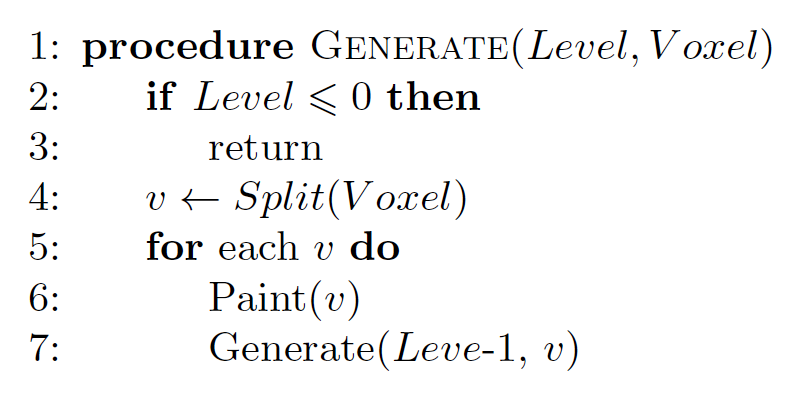
\includegraphics[width=0.95\linewidth]{pic04}
\label{figure02}
\end{figure}
\end{frame}

\begin{frame}
\frametitle{Generation Algorithm}
\begin{figure}[h]
  \centering
  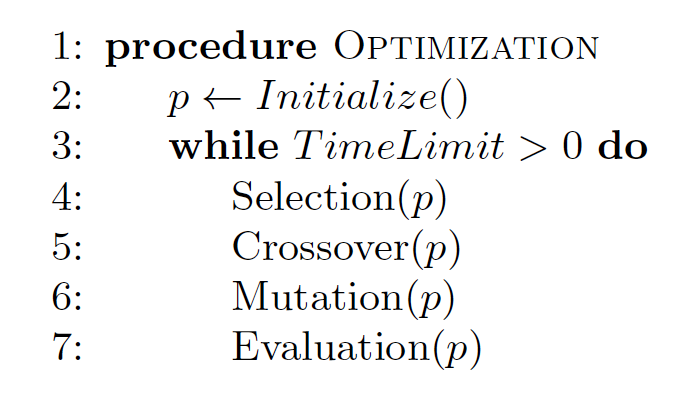
\includegraphics[width=0.95\linewidth]{pic05}
\label{figure03}
\end{figure}
\end{frame}

\begin{frame}
\frametitle{Optimization Specifics}
\begin{itemize}
  \item GA individuals are sets of 32 transition matrices
  \item Parents for the crossover are appointed by tournament selection with arity of two
  \item Uniform crossover is used
  \item Random change of a color is used as mutation
  \item Euclidean distance between generated fractal and target shape is used as fitness function
  \item Time limit is used as stopping criteria
\end{itemize}
\end{frame}

\section{Experiments and Results}

\begin{frame}
\center \huge{Experiments and Results}
\end{frame}

\begin{frame}
\frametitle{Experimental Setup}
\begin{itemize}
  \item All experiments are done in Java as a programming language
  \item Apache Genetic Algorithms Framework is used for the optimization
  \item Printing in 3D - JavaSCAD is used as 3D visualization tool
  \item The source code is available at: github.com/TodorBalabanov/Jack-Hodkinson-3D-Fractal
\end{itemize}
\end{frame}

\begin{frame}
\frametitle{Genetic Algorithm Parameters}
\begin{table}[h!]
\centering
\label{table01}
\begin{tabular*}{\textwidth}{|c@{\extracolsep{\fill}}|c|}
\hline 
\textbf{Parameter} & \textbf{Value} \\
\hline
\hline
elitism rate & 0.10 \\
\hline
crossover rate & 0.90 \\
\hline
mutation rate & 0.01 \\
\hline
number of individuals & 37 \\
\hline
number of variables &  864 \\
\hline
optimization minutes & 30 \\
\hline
\end{tabular*}
\end{table}
\end{frame}

\begin{frame}
\frametitle{Target Object}
\begin{figure}[h]
  \centering
  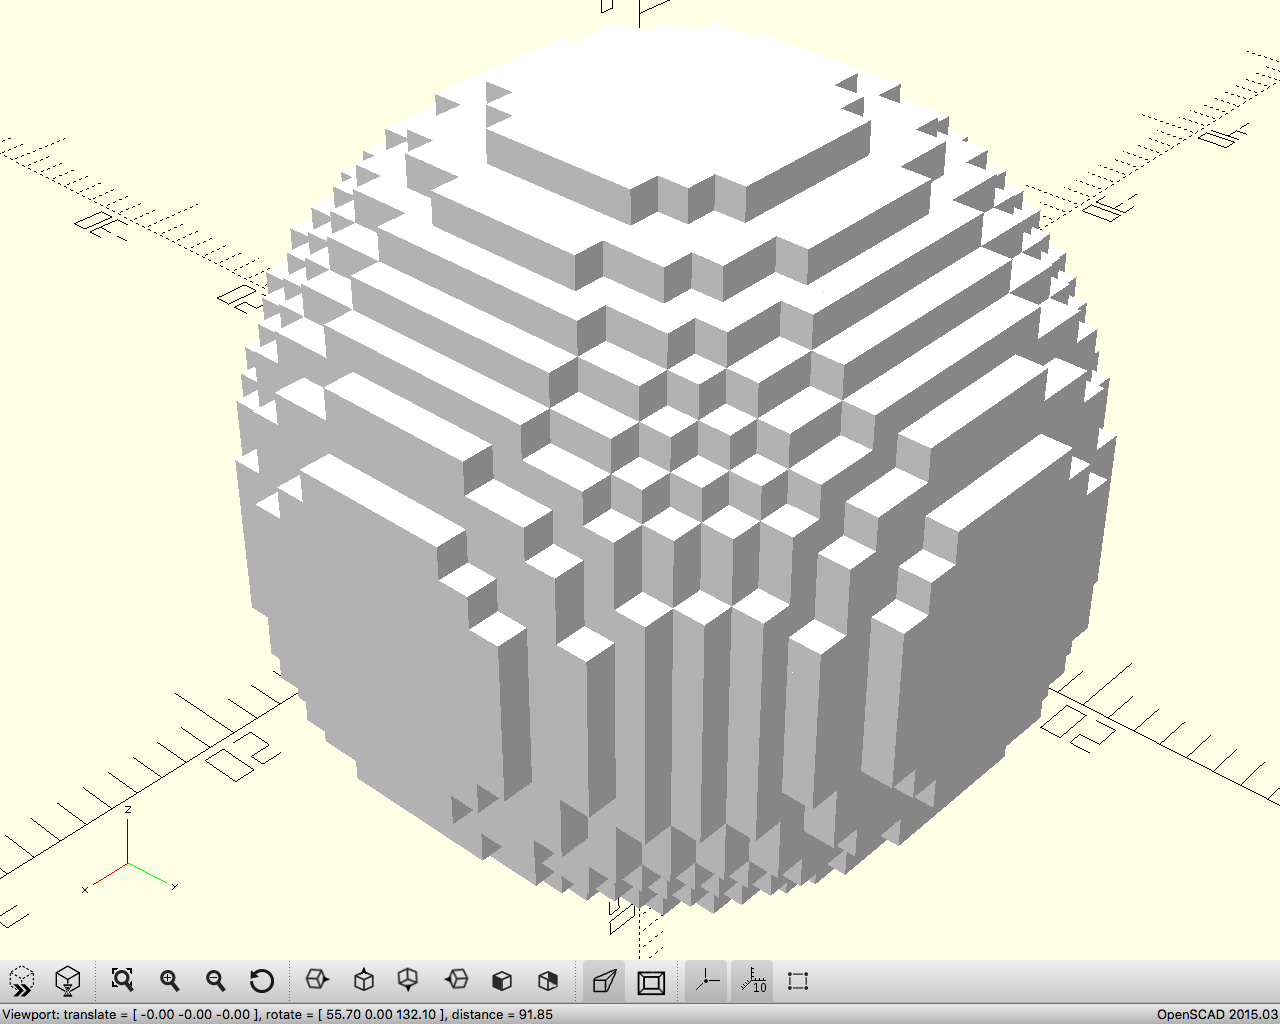
\includegraphics[width=0.75\linewidth]{pic02}
\label{figure04}
\end{figure}
\end{frame}

\begin{frame}
\frametitle{Intermediate Objects}
\begin{figure}[h]
  \centering
  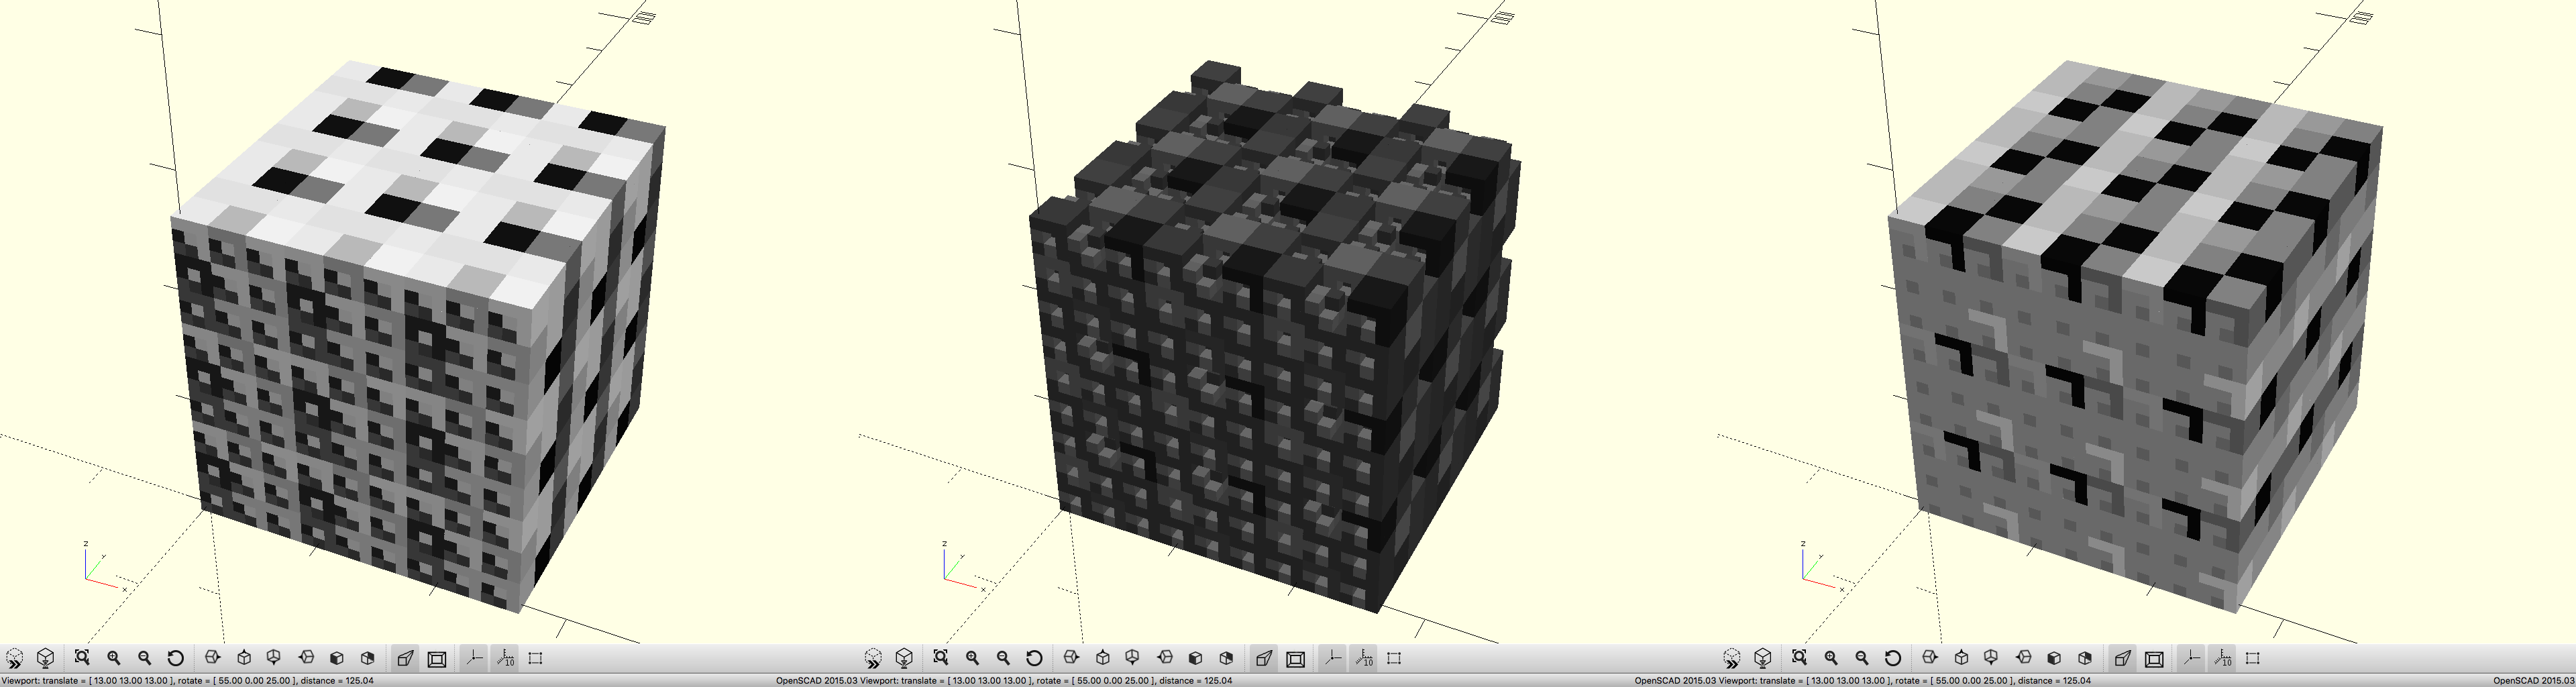
\includegraphics[width=1.00\linewidth]{pic03}
\label{figure05}
\end{figure}
\end{frame}

\section{Conclusions}

\begin{frame}
\center \huge{Conclusions}
\end{frame}

\begin{frame}
\frametitle{Concluding Remarks}
\begin{itemize}
  \item Such optimization is a time consuming process
  \item Virtual 3D objects could be better presented as real world objects with 3D scanner and 3D color printer
  \item A possible application of the presented ideas is compression of 3D images
  \item As further research, parallelization of the genetic algorithm can lead to optimization speed-up
\end{itemize}
\end{frame}

\begin{frame}
\frametitle{Questions and Answers}
\center \huge{Thank you for the attention!}
\end{frame}

\end{document}
